\documentclass[spanish,a4paper,14pt,oneside]{extreport}

%%%%%%%%%%%%%%%%%%%%%%%%%%%%%%%%%%%%%%%%%%%%%%%%%%%%%%%%%%%%%%%%%%%%%%%%%%%%%%%
\usepackage[dvips]{graphicx}
\usepackage[dvips]{epsfig}
\usepackage[utf8]{inputenc}
\usepackage[spanish]{babel}
\usepackage{alltt}
\usepackage{algorithm}
\usepackage{algorithmic}
\usepackage{multirow}
\usepackage[top=2cm, bottom=2cm, left=2cm, right=2cm]{geometry}
\usepackage[usenames]{xcolor}
\usepackage{wrapfig}
\usepackage{caption}
%%%%%%%%%%%%%%%%%%%%%%%%%%%%%%%%%%%%%%%%%%%%%%%%%%%%%%%%%%%%%%%%%%%%%%%%%%%%%%%

\newcommand{\SONY}{{\sc Sony}}
\newcommand{\MICROSOFT}{{\sc Microsoft}}
\newcommand{\GCC}{\textsf{\textsc{G}CC}}
\newcommand{\INTEL}{\textsf{\textsc{I}ntel}}

%%% Traducimos el pseudocodigo
\renewcommand{\algorithmicwhile}{\textbf{mientras}}
\renewcommand{\algorithmicend}{\textbf{fin}}
\renewcommand{\algorithmicdo}{\textbf{hacer}}
\renewcommand{\algorithmicif}{\textbf{si}}
\renewcommand{\algorithmicthen}{\textbf{entonces}}
\renewcommand{\algorithmicrepeat}{\textbf{repetir}}
\renewcommand{\algorithmicuntil}{\textbf{hasta que}}
\renewcommand{\algorithmicelse}{\textbf{en otro caso}}
\renewcommand{\algorithmicfor}{\textbf{para}}

%\newcommand{\RETURN}{\textbf{retornar} }
\newcommand{\RET}{\STATE \textbf{retornar} }
\newcommand{\TO}{\textbf{hasta} }
\newcommand{\AND}{\textbf{y} }
\newcommand{\OR}{\textbf{o} }

%%%%%%%%%%%%%%%%% Creamos un entorno para listar código fuente %%%%%%%%%%%%%%%
\newenvironment{sourcecode}
{\begin{list}{}{\setlength{\leftmargin}{1em}}\item\scriptsize\bfseries}
{\end{list}}

\newenvironment{littlesourcecode}
{\begin{list}{}{\setlength{\leftmargin}{1em}}\item\tiny\bfseries}
{\end{list}}

\newenvironment{summary}
{\par\noindent\begin{center}\textbf{Abstract}\end{center}\begin{itshape}\par\noindent}
{\end{itshape}}

\newenvironment{keywords}
{\begin{list}{}{\setlength{\leftmargin}{1em}}\item[\hskip\labelsep \bfseries Keywords:]}
{\end{list}}

\newenvironment{palabrasClave}
{\begin{list}{}{\setlength{\leftmargin}{1em}}\item[\hskip\labelsep \bfseries Palabras clave:]}
{\end{list}}


%%%%%%%%%%%%%%%%%%%%%%%%%%%%%%%%%%%%%%%%%%%%%%%%%%%%%%%%%%%%%%%%%%%%%%%%%%%%%%%
% Format
%%%%%%%%%%%%%%%%%%%%%%%%%%%%%%%%%%%%%%%%%%%%%%%%%%%%%%%%%%%%%%%%%%%%%%%%%%%%%%%
%\usepackage{showframe}
%\marginparwidth 0mm
%%\topmargin -4 mm
%\topmargin -21 mm
%\headheight 10 mm
%\headsep 10 mm

%\textheight 229 mm
%\textheight 246 mm

%\oddsidemargin -5.4 mm
%\evensidemargin -5.4 mm
%\oddsidemargin 5 mm
%\evensidemargin 5 mm

%\oddsidemargin -3 mm
%\evensidemargin -3 mm

%\textwidth 17 cm
%\textwidth 15 cm
%\columnsep 10 mm

\input{amssym.def}

%%%%%%%%%%%%%%%%%%%%%%%%%%%%%%%%%%%%%%%%%%%%%%%%%%%%%%%%%%%%%%%%%%%%%%%%%%%%%%%

\begin{document}

%%%%%%%%%%%%%%%%%%%%%%%%%%%%%%%%%%%%%%%%%%%%%%%%%%%%%%%%%%%%%%%%%%%%%%%%%%%%%%%
% First Page
%%%%%%%%%%%%%%%%%%%%%%%%%%%%%%%%%%%%%%%%%%%%%%%%%%%%%%%%%%%%%%%%%%%%%%%%%%%%%%%

\pagestyle{empty}
\thispagestyle{empty}


\newcommand{\HRule}{\rule{\linewidth}{1mm}}
\setlength{\parindent}{0mm}
\setlength{\parskip}{10pt}

\vspace*{\stretch{0.5}}

\begin{center}

\includegraphics[scale=0.8]{images/logo_vertical}\\[10mm]
{\Huge Trabajo de Fin de Grado}
\end{center}

\HRule
\begin{flushright}
        {\Huge Visión artificial aplicada a la robótica} \\[2.5mm]
        {\Large \textit{Artificial vision applied to robotics} .} \\[5mm]
        {\Large Miguel Ángel Delgado Hernández} \\[5mm]


\end{flushright}
\HRule
\vspace*{\stretch{2}}
\begin{center}
  \Large La Laguna, \today
\end{center}

\setlength{\parindent}{5mm}

%%%%%%%%%%%%%%%%%%%%%%%%%%%%%%%%%%%%%%%%%%%%%%%%%%%%%%%%%%%%%%%%%%%%%%%%%%%%%%%
% Signature page (add the official stamp)
%%%%%%%%%%%%%%%%%%%%%%%%%%%%%%%%%%%%%%%%%%%%%%%%%%%%%%%%%%%%%%%%%%%%%%%%%%%%%%%
\newpage
%\cleardoublepage
\thispagestyle{empty}

D. {\bf Jonay Tomás Toledo Carrillo}, con N.I.F. 78.698.554-Y
profesor
Contratado Doctor de Universidad
adscrito al Departamento
de Ing. Informática y de Sistemas
de la Universidad de La Laguna, como tutor

\bigskip
\bigskip
{\bf C E R T I F I C A}

\bigskip
\bigskip
\bigskip
Que la presente memoria titulada:

\bigskip
``{\it Visión artificial aplicada a la robótica.}''

\bigskip
\bigskip
\bigskip

\noindent ha sido realizada bajo su dirección por D. {\bf Miguel Ángel Delgado Hernández},
con N.I.F. 54.112.876-V.

\bigskip
\bigskip

Y para que así conste, en cumplimiento de la legislación vigente y a los efectos
oportunos firman la presente en La Laguna a \today

%\cleardoublepage
\newpage
%%%%%%%%%%%%%%%%%%%%%%%%%%%%%%%%%%%%%%%%%%%%%%%%%%%%%%%%%%%%%%%%%%%%%%%%%%%%%%%
\thispagestyle{empty}

{ \flushright

\begin{LARGE}
Agradecimientos
\end{LARGE}

\hspace{3mm}

\begin{large}


\hspace{3mm}
XXX

\hspace{3mm}
XXX


\hspace{3mm}
XXX


\hspace{3mm}
XXX


\end{large}

}

%%%%%%%%%%%%%%%%%%%%%%%%%%%%%%%%%%%%%%%%%%%%%%%%%%%%%%%%%%%%%%%%%%%%%%%%%%%%%%%%%
\newpage

\begin{huge}
Licencia
\end{huge}

\begin{center}

\includegraphics[scale=1.5]{images/by-nc-sa_88x31}\\[10mm]
{\Large \copyright~Esta obra está bajo una licencia de Creative Commons Reconocimiento-NoComercial-CompartirIgual 4.0 Internacional.
}
\end{center}

%%%%%%%%%%%%%%%%%%%%%%%%%%%%%%%%%%%%%%%%%%%%%%%%%%%%%%%%%%%%%%%%%%%%%%%%%%%%%%%
\newpage  %\cleardoublepage
\begin{abstract}
{\em

El objetivo de este trabajo ha sido ....
%
bla, bla, bla
%
bla, bla, bla
%
bla, bla, bla

\bigskip
Las cámaras son uno de los sensores que pueden dar una información mas
rica del entorno para un robot. En este proyecto se plantea la utilización de
cámaras y de sistemas estereoscópicos de dos cámaras para la detección de
obstáculos y su posterior esquiva.

\bigskip
La competencia [E6], que figura en la guía docente, indica que en la memoria del trabajo se ha de incluir:
antecedentes, problemática o estado del arte, objetivos, fases y desarrollo del proyecto,
conclusiones, y líneas futuras.

\bigskip
Se ha incluido el apartado de 'Licencia' con todas las posibles licencias abiertas (Creative Commons).
En el caso en que se decida hacer público el contenido de la memoria, habrá que elegir una de ellas
(y borrar las demás).
La decisión de hacer pública o no la memoria se indica en el momento de subir la memoria a la Sede Electrónica de la ULL, paso necesario en el proceso de presentación del TFG.

\bigskip
El documento de memoria debe tener un máximo de 50 páginas.

\bigskip
No se deben dejar páginas en blanco al comenzar un capítulo, ya que
el documento no está pensado para se impreso sino visionado
con un lector de PDFs.

\bigskip
También es recomendable márgenes pequeños ya que, al firmar digitalmente por
la Sede, se coloca un marco alrededor del texto original.


\bigskip
El tipo de letra base ha de ser de 14ptos.
}

\begin{palabrasClave}
Palabra reservada1, Palabra reservada2, ...
\end{palabrasClave}

\end{abstract}
%%%%%%%%%%%%%%%%%%%%%%%%%%%%%%%%%%%%%%%%%%%%%%%%%%%%%%%%%%%%%%%%%%%%%%%%%%%%%%%

%%%%%%%%%%%%%%%%%%%%%%%%%%%%%%%%%%%%%%%%%%%%%%%%%%%%%%%%%%%%%%%%%%%%%%%%%%%%%%%
\newpage  %\cleardoublepage
\begin{summary}
{\em

Here should be the abstract in a foreing language...

}

\begin{keywords}
Keyword1, Keyword2, Keyword3, ...
\end{keywords}

\end{summary}
%%%%%%%%%%%%%%%%%%%%%%%%%%%%%%%%%%%%%%%%%%%%%%%%%%%%%%%%%%%%%%%%%%%%%%%%%%%%%%%

%%%%%%%%%%%%%%%%%%%%%%%%%%%%%%%%%%%%%%%%%%%%%%%%%%%%%%%%%%%%%%%%%%%%%%%%%%%%%%%
\newpage{\pagestyle{empty}}
\thispagestyle{empty}

%%%%%%%%%%%%%%%%%%%%%%%%%%%%%%%%%%%%%%%%%%%%%%%%%%%%%%%%%%%%%%%%%%%%%%%%%%%%%%%


\pagestyle{myheadings} %my head defined by markboth or markright
% No funciona bien \markboth sin "twoside" en \documentclass, pero al
% ponerlo se dan un montón de errores de underfull \vbox, con lo que no se
% ha puesto.
\markboth{Miguel Ángel Delgado Hernández}{Visión artificial aplicada a la robótica}

%%%%%%%%%%%%%%%%%%%%%%%%%%%%%%%%%%%%%%%%%%%%%%%%%%%%%%%%%%%%%%%%%%%%%%%%%%%%%%%
%Numeracion en romanos
\renewcommand{\thepage}{\roman{page}}
\setcounter{page}{1}

%%%%%%%%%%%%%%%%%%%%%%%%%%%%%%%%%%%%%%%%%%%%%%%%%%%%%%%%%%%%%%%%%%%%%%%%%%%%%%%

\tableofcontents

%%%%%%%%%%%%%%%%%%%%%%%%%%%%%%%%%%%%%%%%%%%%%%%%%%%%%%%%%%%%%%%%%%%%%%%%%%%%%%%
\newpage{\pagestyle{empty}}

\listoffigures

%%%%%%%%%%%%%%%%%%%%%%%%%%%%%%%%%%%%%%%%%%%%%%%%%%%%%%%%%%%%%%%%%%%%%%%%%%%%%%%
\newpage{\pagestyle{empty}}

\listoftables

%%%%%%%%%%%%%%%%%%%%%%%%%%%%%%%%%%%%%%%%%%%%%%%%%%%%%%%%%%%%%%%%%%%%%%%%%%%%%%%
\newpage{\pagestyle{empty}}

%%%%%%%%%%%%%%%%%%%%%%%%%%%%%%%%%%%%%%%%%%%%%%%%%%%%%%%%%%%%%%%%%%%%%%%%%%%%%%%
%Numeracion a partir del capitulo I
\renewcommand{\thepage}{\arabic{page}}
\setcounter{page}{1}


\chapter{Introducción}
\label{chapter:intro}

%%%%%%%%%%%%%%%%%%%%%%%%%%%%%%%%%%%%%%%%%%%%%%%%%%%%%%%%%%%%%%%%%%%%%%%%%%%%%%%%
% Chapter 1: Introducción
%%%%%%%%%%%%%%%%%%%%%%%%%%%%%%%%%%%%%%%%%%%%%%%%%%%%%%%%%%%%%%%%%%%%%%%%%%%%%%%%

%+++++++++++++++++++++++++++++++++++++++++++++++++++++++++++++++++++++++++++++++

%+++++++++++++++++++++++++++++++++++++++++++++++++++++++++++++++++++++++++++++++


% \textcolor{red}{text}
%+++++++++++++++++++++++++++++++++++++++++++++++++++++++++++++++++++++++++++++++
\section{Antecedentes}
\label{1:sec:1}

Puntos clave: robots, sistemas guiados, camaras estereoscopicas, deteccion de
obstaculos

Las cámaras son uno de los sensores que pueden dar una información mas
rica del entorno para un robot. En este proyecto se plantea la utilización de
cámaras y de sistemas estereoscópicos de dos cámaras para la detección de
obstáculos y su posterior esquiva.


%+++++++++++++++++++++++++++++++++++++++++++++++++++++++++++++++++++++++++++++++
\section{Estado del arte}
\label{1:sec:2}


%+++++++++++++++++++++++++++++++++++++++++++++++++++++++++++++++++++++++++++++++
\section{Objetivo}
\label{1:sec:3}

El tema central de este proyecto es muy ambicioso, de este modo, es necesario
poder realizar una distinción entre el objetivo principal y los objetivos
específicos que lo rodean.

%--------------------------------------
\subsection{Objetivo general}

\textcolor{red}{¿Detección y esquiva o reconstrucción del mapa?}

El objetivo principal de este Trabajo de Fin de Grado es poder integrar el uso
de un sistema estereoscópico de dos cámaras en un robot, para la detección y
posteriormente esquiva de los obstáculos que se encuentren.

%--------------------------------------
\subsection{Objetivos específicos}

Los objetivos específicos que componen el proyecto son:
% \newline
\begin{itemize}
\item Uso de una cámara comercial de entretenimiento en un proyecto de
investigación.
\item Reconstrucción de un mapa tridimensional a partir de las imágenes
recogidas por las cámaras.
\item Integración de cámaras estereoscópicas junto a otros sistemas de detección
% \section{Sección Tres}
de obstáculos.
\end{itemize}


%+++++++++++++++++++++++++++++++++++++++++++++++++++++++++++++++++++++++++++++++
% \label{1:sec:3}
% \begin{itemize}
%   \item Item 1
%   \item Item 2
%   \item Item 3
% \end{itemize}
% Bla, bla, bla

%+++++++++++++++++++++++++++++++++++++++++++++++++++++++++++++++++++++++++++++++
% \section{Sección Cuatro}
%   \label{1:sec:4}
%
% Bla, bla, bla

%+++++++++++++++++++++++++++++++++++++++++++++++++++++++++++++++++++++++++++++++
% \begin{figure}[!th]
% \begin{center}
% \includegraphics[width=0.5\textwidth]{images/arbolbinario.eps}
% \caption{Ejemplo}
% \label{fig:ArbolBinario}
% \end{center}
% \end{figure}
%+++++++++++++++++++++++++++++++++++++++++++++++++++++++++++++++++++++++++++++++


%%%%%%%%%%%%%%%%%%%%%%%%%%%%%%%%%%%%%%%%%%%%%%%%%%%%%%%%%%%%%%%%%%%%%%%%%%%%%%%

\chapter{Conceptos}
\label{chapter:dos}

%%%%%%%%%%%%%%%%%%%%%%%%%%%%%%%%%%%%%%%%%%%%%%%%%%%%%%%%%%%%%%%%%%%%%%%%%%%%%%%%
% Chapter 2: Conceptos
%%%%%%%%%%%%%%%%%%%%%%%%%%%%%%%%%%%%%%%%%%%%%%%%%%%%%%%%%%%%%%%%%%%%%%%%%%%%%%%%

%+++++++++++++++++++++++++++++++++++++++++++++++++++++++++++++++++++++++++++++++
En este capítulo se abordarán todos aquellos conceptos teóricos que han surgido
a lo largo del proyecto y son necesarios para entender correctamente la línea
del trabajo.


%+++++++++++++++++++++++++++++++++++++++++++++++++++++++++++++++++++++++++++++++
\section{Visión artificial}
\label{2:sec:1}
% https://campusvirtual.ull.es/1516/course/view.php?id=202
% https://es.wikipedia.org/wiki/Visi%C3%B3n_artificial
% https://en.wikipedia.org/wiki/Computer_vision
% J. GONZÁLEZ JIMÉNEZ, "Visión Por Computador", Editorial Paraninfo. 2000

La visión artificial por computador, es la disciplina científica que se basa en
la adquisición, procesamiento y análisis de las imágenes que se toman del mundo
real, con el objetivo de obtener información relevante acerca de ellas:
detección de objetos, seguimiento del movimiento, reconocimiento de eventos,
etc. Un ejemplo que podemos ver en nuestro día a día, es la detección de caras
en una escena capturada por una cámara digital o smartphone, mediante el uso de
téncicas de reconocimiento de patrones.

Al igual que sucede en otras áreas de la inteligencia artificial, la visión
artificial tiene como objetivo principal obtener la información explícita y el
significado de la realidad de la misma manera que lo haría un ser biológico.

El avance progresivo del hardware con nuevos procesadores digitales de señales
(DSP) y unidades de procesamiento gráfico (GPU), junto con nuevas tecnologías y planteamientos de cómputo como la computación paralela, ha permitido que en los
últimos años se haya podido implementar nuevos algortimos más rápidos y
eficientes, necesarios para ser utilizados en ámbitos críticos, como sistemas
en tiempo real.

%--------------------------------------
\subsection{Objetivos}

\textcolor{red}{Lorem ipsum dolor sit amet, consectetur adipisicing elit, sed do
 eiusmod tempor incididunt ut labore et dolore magna aliqua. Ut enim ad minim 
 veniam, quis nostrud exercitation ullamco laboris nisi ut aliquip ex ea commodo 
 consequat. Duis aute irure dolor in reprehenderit in voluptate velit esse cillum
 dolore eu fugiat nulla pariatur. Excepteur sint occaecat cupidatat non proident,
 sunt in culpa qui officia deserunt mollit anim id est laborum.}

\textcolor{red}{Lorem ipsum dolor sit amet, consectetur adipisicing elit, sed do
 eiusmod tempor incididunt ut labore et dolore magna aliqua. Ut enim ad minim 
 veniam, quis nostrud exercitation ullamco laboris nisi ut aliquip ex ea commodo 
 consequat. Duis aute irure dolor in reprehenderit in voluptate velit esse cillum
 dolore eu fugiat nulla pariatur. Excepteur sint occaecat cupidatat non proident,
 sunt in culpa qui officia deserunt mollit anim id est laborum.}

%--------------------------------------
\subsection{Dificultades}
La capacidad visual es uno pilares de la inteligencia humana. Su implementación
en la rotótica supone también un importante avance en la inteligencia artificial.
Sin embargo, mientras que la percepción visual es algo innato y cotidiano para
nosotros, la visión artificial es muy compleja y conlleva muchas dificultades.
Entre las principales dificultades, destacan:

\begin{itemize}
  \item \textbf{Mundo tridimensional:} mientras que las imágenes que se obtienen
  con una cámara son bidimensionales, el mundo que nos rodea no. Es necesario 
  realizar las transformaciones correspondientes para obtener valores correctos.
  \item \textbf{Zonas de interés:} se necesita extraer elementos de información 
  sutiles en imágenes complejas, por lo que entre tanta información es necesario
  reconocer formas, colores, etc.
  \item \textbf{Carácter dinámico de las escenas:} el mundo está vivo, por lo
  que en las imágenes que se toman muchos elementos están en movimiento. Por 
  otro lado, otros factores como luminosidad, contraste, foco... pueden marcar
  una importante diferencia, y por desgracia, estos factores son variables, no
  se pueden controlar.
\end{itemize}

%--------------------------------------
% \subsection{Reconocimiento}

% Detección de objetos

%--------------------------------------
% \subsection{Motion Analysis}

% Video grabación de imágenes de seguridad

%--------------------------------------
% \subsection{Reconstrucción}


%+++++++++++++++++++++++++++++++++++++++++++++++++++++++++++++++++++++++++++++++
\section{Visión estéreo}
\label{2:sec:2}
% http://vision.deis.unibo.it/~smatt/Seminars/StereoVision.pdf
% http://www.cesfelipesegundo.com/revista/articulos2011/Guerrero,%20J.M.pdf

La visión estereoscópica o visión estéreo, es la técnica capaz de extraer
información tridimensional (profundidad) a partir de la posición relativa de un
objeto en imágenes bidimensionales al ser observado desde distintos ángulo por
dos o más cámaras separadas a una cierta distancia.

%--------------------------------------
\subsection{Adquisición}

Usando dos cámaras, el procedimiento a seguir para la adquisición del entorno es
capturar dos imágenes de una misma escena, desde dos cámaras separadas
ligeramente. De esta forma, las imágenes obtenidas, también tendrán un pequeño 
desplazamiento entre sí.

De manera más formal, se obtiene que para cada imagen capturada por las
cámaras, un objeto está en puntos diferentes del plano. Esta triangulazión
entre el punto P y Q y el origen de referencia, provocan una sensación de
profundidad. Mediante el sistema tradicional de una sola cámara, este punto
estaría en las mismas coordenadas.

\begin{figure}[!th]
  \begin{center}
    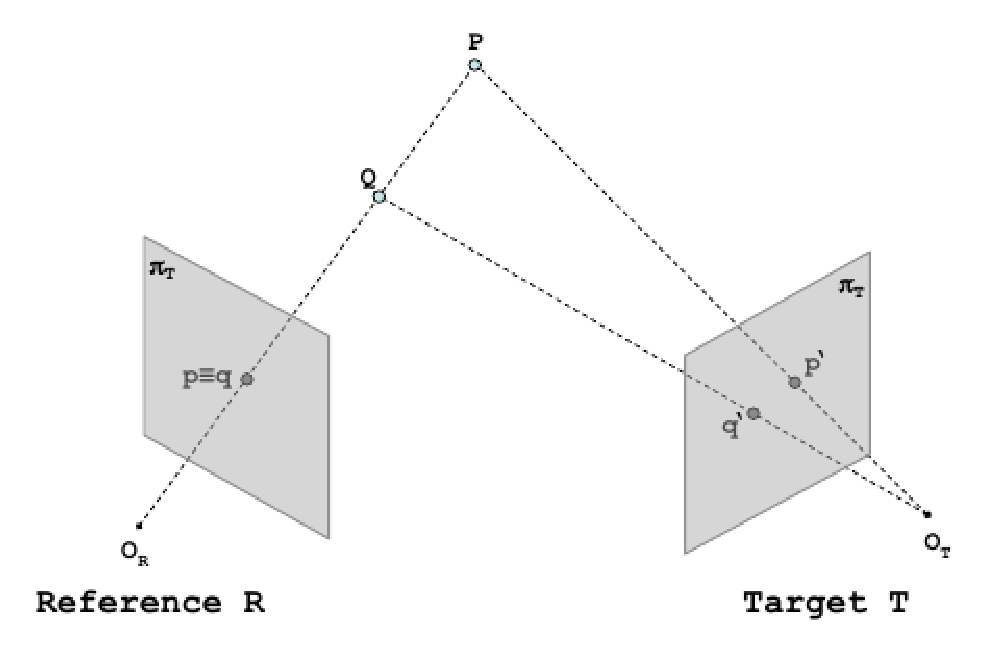
\includegraphics[width=0.7\textwidth]{images/cap2/VisionEstereo.eps}
    \caption{Diferencias entre una y dos cámaras}
    \label{fig:VisionEstereo}
  \end{center}
\end{figure}

Con estos datos, se pueden poner en correspondencia cada punto de ambas
imágenes, para obtener una imagen de disparidad (más información en la sección 
2.2.4).

%--------------------------------------
\subsection{Geometría de las cámaras}
% https://en.wikipedia.org/wiki/Parallax
% http://www.cesfelipesegundo.com/revista/articulos2011/Guerrero,%20J.M.pdf
En función de la posición relativa de las cámaras entre sí, se pueden apreciar
dos métodos principales:

\begin{itemize}
  \item \textbf{Visión paralela:} las cámaras están paralelas entre sí y están
  separadas por una línea horizonal (línea base). El objetivo que visualiza
  cada cámara es perpendicular respecto a la línea base, mientras que las
  líneas de correspondencia que unen los puntos de una imagen respecto a la otra
  son horizontales.

  \begin{minipage}{\linewidth}
      \centering
      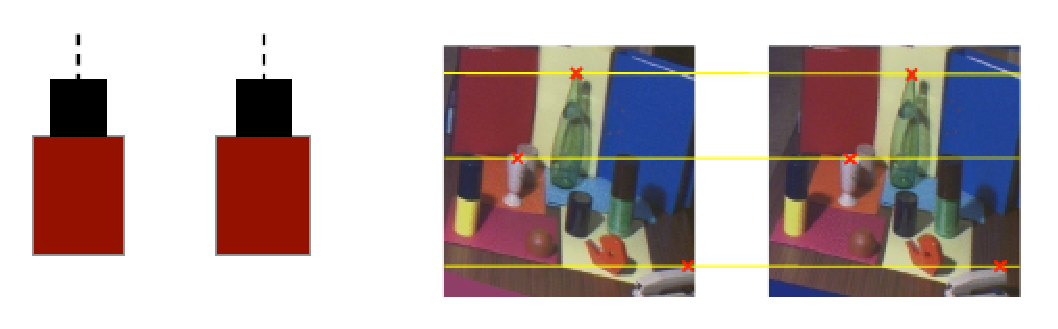
\includegraphics[width=0.7\textwidth]{images/cap2/VisionParalela.eps}
      \captionof{figure}{Visión paralela}
      \label{fig:VisionParalela}
  \end{minipage}

  \item \textbf{Visión cruzada:} las cámaras no están paralelas entre sí, tienen
  una inclinación de tal forma que el objetivo de cada cámara apunta hacia el
  lado contrario de una imagen. Por lo que los ejes ópticos se cruzan entre sí.
  Las líneas de correspondencia, también tienen sufren una inclinación.

  \begin{minipage}{\linewidth}
      \centering
      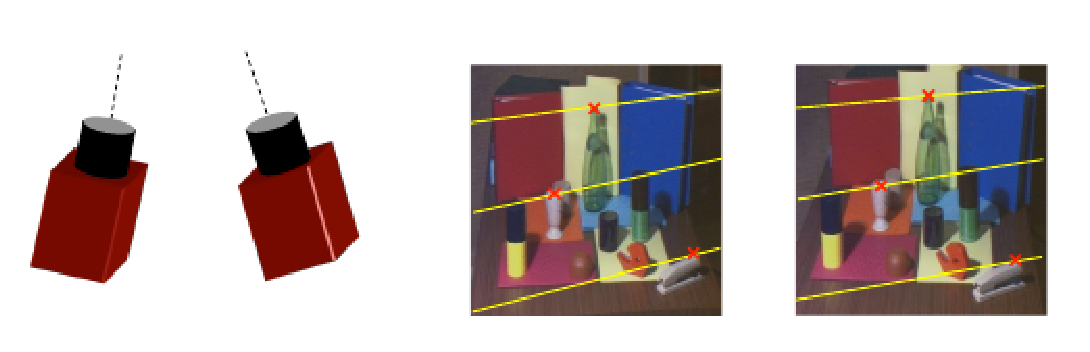
\includegraphics[width=0.7\textwidth]{images/cap2/VisionCruzada.eps}
      \captionof{figure}{Visión cruzada}
      \label{fig:VisionCruzada}
  \end{minipage}
\end{itemize}

% http://vfxio.com/PDFs/Parallel_vs_Converged.pdf
La visión cruzada tiene la desventaja de distorsionar las imágenes capturadas.
En la figura 2.4 se puede observar este efecto al fotografíar un muro de
ladrillos. Sin embargo, dependiendo del tipo de escena que se capture, esta
distorsión puede suponer un problema o no.

\begin{figure}[!th]
  \begin{center}
    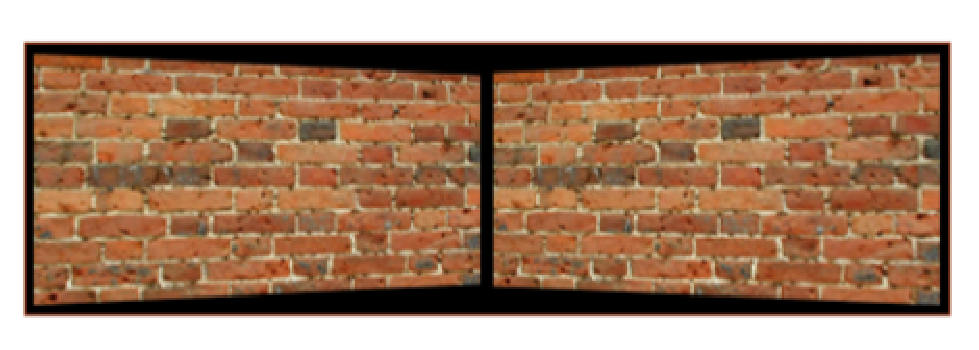
\includegraphics[width=0.5\textwidth]{images/cap2/VisionCruzadaMuro.eps}
    \caption{Muro distorsionado por visión cruzada}
    \label{fig:VisionCruzadaMuro}
  \end{center}
\end{figure}

La visión paralela por su parte, no distorsiona las imágenes capturadas, pero
también cuenta con otra serie de problemas. \textcolor{red}{Lorem ipsum dolor sit amet, consectetur adipisicing elit, sed do eiusmod tempor incididunt ut labore et dolore magna aliqua. Ut enim ad minim veniam, quis nostrud exercitation ullamco laboris nisi ut aliquip ex ea commodo consequat. Duis aute irure dolor in reprehenderit in voluptate velit esse cillum dolore eu fugiat nulla pariatur. Excepteur sint occaecat cupidatat non proident, sunt in culpa qui officia deserunt mollit anim id est laborum.}

%--------------------------------------
\subsection{Rectificación}
% https://en.wikipedia.org/wiki/Image_rectification

%--------------------------------------
\subsection{Disparidad}
% http://es.slideshare.net/RicardoSnchezCastill/vision-artificial-49264591
% http://stackoverflow.com/questions/17607312/difference-between-disparity-map-and-disparity-image-in-stereo-matching
% http://iie.fing.edu.uy/publicaciones/2005/Lec05a/Lec05a.pdf
La disparidad de dos imágenes establece la correspondencia entre los píxeles o
características que existen entre ambas para obtener la profundidad de la
escena. Conociendo la geometría del entorno y la cámara, de forma general, se
realiza una triangulación entre cada punto de las imágenes para obtener la
disparidad.

Metodos:


El objetivo final es poder construir una \textbf{imagen o mapa de disparidad}







% Disparidad....

% http://www.cesfelipesegundo.com/revista/articulos2011/Guerrero,%20J.M.pdf
% http://dmi.uib.es/~abasolo/cursorealidad/paco/Estereoscopia.html
%--------------------------------------
\subsection{Aplicaciones}
% https://www.ptgrey.com/tan/10570
La visión artificial resulta de gran utilidad en diferentes áreas de aplicación,
tanto en acciones repetitivas como peligrosas:

\begin{itemize}
  \item \textbf{Inspección y ensamblaje industrial:} el proyecto "Randon Bin
  Picking" (RBP) hace uso de visión estéreo para la búsqueda de piezas entre
  objetos de todo tipo para su rápida recuperación.
  % http://www.worldscientific.com/doi/suppl/10.1142/8766/suppl_file/8766_chap01.pdf
  \item \textbf{Apoyo en el diagnóstico médico:} en las últimas décadas la
  visión artificial se ha hecho un importante en la medicina para detectar,
  analizar y reconstruir la información obtenida.
  % http://www.ri.cmu.edu/pub_files/pub4/matthies_larry_2007_1/matthies_larry_2007_1.pdf
  \item \textbf{Exploración espacial:} en el proyecto de exploración Mars Rover
  (Mars Exploration Rover Mission) tiene como objetivo explorar la superficie
  de Marte en busca de rocas u otros elementos que prueben la existencia de
  agua.
  \item \textbf{Seguimiento (Tracking):} se hace uso en innumerables situaciones
  de carácter estadístico como contar el número o de en áreas de vigilancia y
  seguridad monitorizando trayectorias.
\end{itemize}


%+++++++++++++++++++++++++++++++++++++++++++++++++++++++++++++++++++++++++++++++
\section{Odometría}
\label{2:sec:3}

%--------------------------------------
\subsection{Mecánica}

%--------------------------------------
\subsection{Visual}


%+++++++++++++++++++++++++++++++++++++++++++++++++++++++++++++++++++++++++++++++
\section{Reconstrucción 3D}
\label{2:sec:4}


% http://slipguru.disi.unige.it/OLDslipguru/teaching/Vis2/LUCIDI/class5.pdf

% nube de puntos


%--------------------------------------
\subsection{SLAM}


%+++++++++++++++++++++++++++++++++++++++++++++++++++++++++++++++++++++++++++++++










%%%%%%%%%%%%%%%%%%%%%%%%%%%%%%%%%%%%%%%%%%%%%%%%%%%%%%%%%%%%%%%%%%%%%%%%%%%%%%%
\newpage{\pagestyle{empty}}
\thispagestyle{empty}

\chapter{Recursos y herramientas}
\label{chapter:tres}

%%%%%%%%%%%%%%%%%%%%%%%%%%%%%%%%%%%%%%%%%%%%%%%%%%%%%%%%%%%%%%%%%%%%%%%%%%%%%%%
% Chapter 3: Recursos y herramientas
%%%%%%%%%%%%%%%%%%%%%%%%%%%%%%%%%%%%%%%%%%%%%%%%%%%%%%%%%%%%%%%%%%%%%%%%%%%%%%%

%+++++++++++++++++++++++++++++++++++++++++++++++++++++++++++++++++++++++++++++++
En este capítulo se hablará tanto del hardware como del software utilizado para
realizar el proyecto. A grandes rasgos se integrará la PlayStation Camera en el
sistema Perenquén, utilizando el framework ROS para el funcionamiento de ambos.


%++++++++++++++++++++++++++++++++++++++++++++++++++++++++++++++++++++++++++++++
\section{PlayStation Camera}
\label{3:sec1}
%%%%%%%%%%%%%%%%%%%%%%%%%%%%%%%%%%%%%%%%%%%%%%%%%%%%%%%%%%%%%%%%%%%%%%%%%%%%%%%%
% Chapter 3: Recursos y herramientas
%%%%%%%%%%%%%%%%%%%%%%%%%%%%%%%%%%%%%%%%%%%%%%%%%%%%%%%%%%%%%%%%%%%%%%%%%%%%%%%%

%+++++++++++++++++++++++++++++++++++++++++++++++++++++++++++++++++++++++++++++++
% \section{Playstation Camera}
% \label{3:sec:1}

bla bla bla

%+++++++++++++++++++++++++++++++++++++++++++++++++++++++++++++++++++++++++++++++


%++++++++++++++++++++++++++++++++++++++++++++++++++++++++++++++++++++++++++++++
\section{Perenquén}
\label{3:sec2}
%%%%%%%%%%%%%%%%%%%%%%%%%%%%%%%%%%%%%%%%%%%%%%%%%%%%%%%%%%%%%%%%%%%%%%%%%%%%%%%%
% Chapter 3: Recursos y herramientas
%%%%%%%%%%%%%%%%%%%%%%%%%%%%%%%%%%%%%%%%%%%%%%%%%%%%%%%%%%%%%%%%%%%%%%%%%%%%%%%%

%+++++++++++++++++++++++++++++++++++++++++++++++++++++++++++++++++++++++++++++++
% \section{Perenquén}
% \label{3:sec:2}
Perenquén es el nombre que ha tomado el proyecto de automatización de una silla
de ruedas por el Grupo de Robótica de la Universidad de La Laguna, cuya
filosofía es llevar los progresos conseguidos con el proyecto Verdino, a una
silla de ruedas \cite{ProjectPerenquen}.

\begin{wrapfigure}{l}{0.5\textwidth}
  \vspace{-20pt}
  \begin{center}
    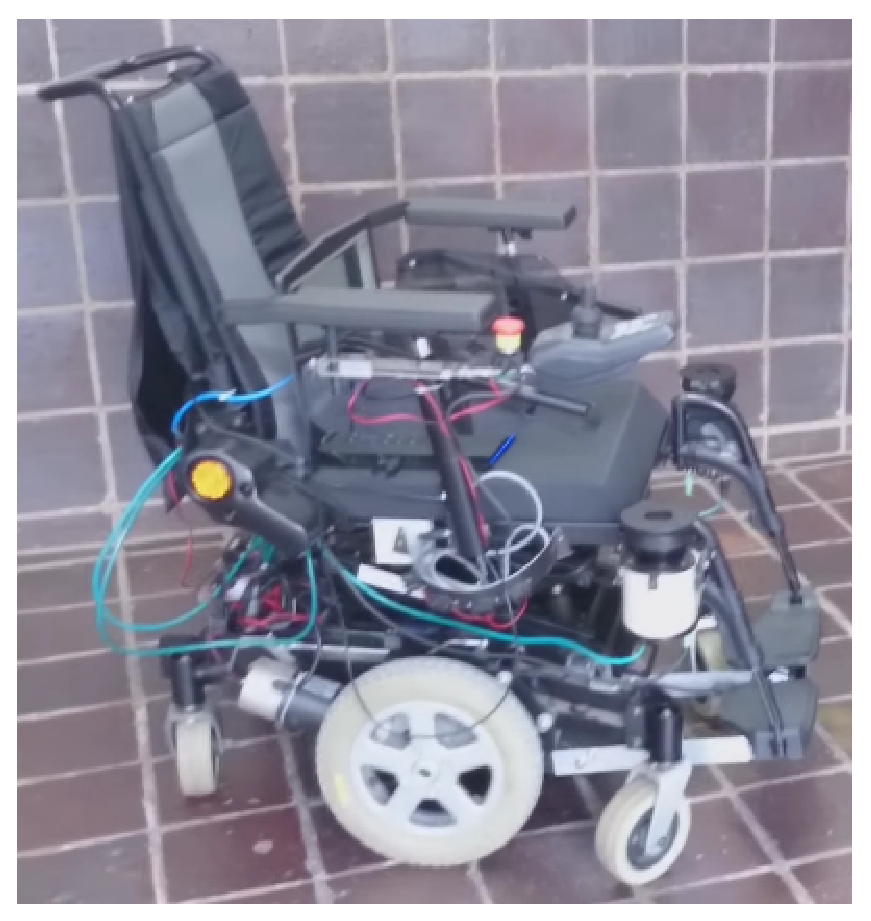
\includegraphics[width=0.48\textwidth]{images/cap3/Perenquen.eps}
  \end{center}
  \vspace{-20pt}
  \caption{Perenquén}
  \vspace{-10pt}
  \label{fig:Perenquen}
\end{wrapfigure}

El objetivo principal de este proyecto es el desplazamiento autónomo de una
silla de ruedas, mediante la detección de obstáculos de un entorno, así como su
localización en el mismo a través de las imágenes capturadas mediante la versión
2.0 de Kinect A diferencia de Verdino, Perenquén intenta ser una alternativa de
bajo coste frente a los sistemas de detección de obstáculo de Verdino.

Actualmente la silla cuenta con el dispositivo Kinect, un sistema de odometría
mecánica, y tres detectores láser (lado izquierdo, lado derecho y posterior) que
hacen posible una detección más precisa de los obstáculos. Sin embargo, Kinect
cuenta con una importante desventaja, y es que no funciona correctamente en
exteriores, tiene un alcance acotado de apenas entre 5 y 10 metros
\cite{PerenquenNoticia}.

%+++++++++++++++++++++++++++++++++++++++++++++++++++++++++++++++++++++++++++++++


%++++++++++++++++++++++++++++++++++++++++++++++++++++++++++++++++++++++++++++++
\section{ROS}
\label{3:sec3}
%%%%%%%%%%%%%%%%%%%%%%%%%%%%%%%%%%%%%%%%%%%%%%%%%%%%%%%%%%%%%%%%%%%%%%%%%%%%%%%%
% Chapter 3: Recursos y herramientas
%%%%%%%%%%%%%%%%%%%%%%%%%%%%%%%%%%%%%%%%%%%%%%%%%%%%%%%%%%%%%%%%%%%%%%%%%%%%%%%%

%+++++++++++++++++++++++++++++++++++++++++++++++++++++++++++++++++++++++++++++++
% \section{ROS}
% \label{3:sec:3}

% http://erlerobotics.com/blog/ros-introduction-es/
% https://www.clearpathrobotics.com/assets/guides/ros/Intro%20to%20the%20Robot%20Operating%20System.html
% http://www.ros.org/about-ros/

% http://www.ros.org/about-ros/
ROS (Robot Operating System) es un framework de código abierto diseñado para
realizar software robótico. Entre las principales funcionalidades destacan una
abstracción del hardware, el control de dispositivos, paso de mensajes entre los
procesos y una gran variedad de herramientas y librerías. Por otra parte ROS
cuenta con un sistema de paquetes, que permite instalar, compilar e incluso
modificar paquetes externos creados por la comunidad.

% http://erlerobotics.com/blog/ros-introduction-es/
El objetivo principal es permitir la abstracción y la simplificación de  muchas de
las tareas que conllevan construir un robot de forma independiente, uno de los
principales problemas que llevan a condenar al fracaso este tipo de proyectos,
mediante el desarrollo de software colaborativo. En definitiva, ROS promueve la
reutilización de código para evitar tener que reinventar la rueda a los
desarrolladores y científicos en cada nuevo proyecto.

% http://www.ros.org/about-ros/
De esta forma, a modo de ejemplo un grupo de desarrolladores puede trabajar e
investigar en la construcción de mapas, mientras que en otra parte del mundo,
otro grupo de expertos puede estar especializado en la localización con el uso
de mapas. Ambos comparten el conocimiento entre ambos y con el resto de la
comunidad para conseguir mejores resultados en conjunto.

% https://en.wikipedia.org/wiki/Robot_Operating_System
El software de ROS se distribuye de la siguiente manera:

\begin{itemize}
  \item Herramientas y lenguajes independientes para construir y distribuir ROS.
  \item Librerías del cliente de ROS que facilitan el desarrollo.
  \item Paquetes que contienen la aplicación del usuario.
\end{itemize}

Tanto las herramientas como las librerías del cliente de ROS están escritas
principalmente en C++ y Python. Las librerías principales de ROS siguen los
principios Unix-like ya que la mayoría de dependencias son proyectos de código
abierto, permitiendo que muchas distribuciones distribuyan las librerías y
paquetes de ROS.

% http://www.ros.org/is-ros-for-me/
ROS ha sido diseñado para ser un sistema distribuido lo más modular posible,
permitiendo que los usuarios puedan utilizar lo justo y necesario, desde los
paquetes del núcleo y la comunidad, hasta utilizar sus propios paquetes
personales. Actualmente ROS cuenta con más de 3000 paquetes públicos en su
ecosistema, siendo difícil conocer cual es el número real de todos los paquetes.
Muchos de estos paquetes ayudan enormemente en la infraestructura de la
comunidad, ofreciendo accesos a drivers de dispositivo, capacidades genéricas en
robótica, algoritmos, herramientas de desarrollo y librerías.

Desde sus inicios, la comunidad de ROS ha crecido considerablemente en todo el
mundo, principalmente en laboratorios de investigación, pero en los últimos
tiempos también en otros sectores comerciales e industriales. Más de 1500
personas participan en las listas de correos, y aproximadamente 6000 personas
colaboran con la documentación oficial y la comunidad de preguntas y respuestas.
Esto implica que más de 30 páginas de la documentación se editen cada día y que
hasta la fecha se hayan abierto más de 13000 preguntas con un porcentaje de
respuesta alto.

%+++++++++++++++++++++++++++++++++++++++++++++++++++++++++++++++++++++++++++++++
\subsection{Historia}

% http://www.ros.org/about-ros/
El origen de ROS se remonta a 2007, cuando Willow Garage pensó en la necesidad
de de diseñar un sistema más flexible y robusto para el desarrollo de robots
después de que en en el laboratorio de inteligencia artificial de la universidad
de Standford es estuvieran realizando diferentes proyectos que integraban el uso
de robots e inteligencia artificial como STandard AI Robot (STAIR) y Personal
Robots (PR).

% https://en.wikipedia.org/wiki/Robot_Operating_System
Varios investigadores contribuyeron y dieorn ideas para lo que sería la base
fundamental del servicio de paquetes de ROS que existe actualmente. En apenas un
año, el proyecto paso a desarollarse por la institución de investigación
robótica Willow Garage, junto con la colaboración de más de veinte
instituciones. Mientras tanto, el uso de una licencia permisiva de código
abierto permitió que de forma gradual ROS se empezará a implementar en
diferentes comunidades de desarrollo robótico. Finalmente, en 2013, ROS se
transferió a la Open Source Robotics Fundation.

Y hasta la fecha se han lanzado las siguientes versiones:

%+++++++++++++++++++++++++++++++++++++++++++++++++++++++++++++++++++++++++++++++
\begin{table}[!ht]
\begin{center}
\begin{tabular}{|p{50mm}|p{35mm}|p{60mm}|} \hline 
\textbf{Nombre} & \textbf{Lanzamiento} & \textbf{Soporte}\\ \hline
Kinectic Kame
&
23/05/2016
&
Soporte hasta 2021
\\
\hline

Jade Turtle
&
23/05/2015
&
Soporte hasta 2017
\\
\hline

Indigo Igloo
&
22/07/2014
&
Soporte hasta 2019
\\
\hline

Hydro Medusa
&
04/09/2013
&
Sin soporte
\\
\hline

Groovy Galapagos
&
31/12/2012
&
Sin soporte
\\
\hline

Fuerte Turtle
&
23/04/2012
&
Sin soporte
\\
\hline

Electric Emys
&
30/08/2011
&
Sin soporte
\\
\hline

Diamondback
&
02/03/2011
&
Sin soporte
\\
\hline

C Turtle
&
02/08/2010
&
Sin soporte
\\
\hline

Box Turtle
&
02/03/2010
&
Sin soporte
\\
\hline


\end{tabular}
\end{center}
\caption{Tabla con versiones de ROS hasta la fecha}
\label{table:playstation-camera}
\end{table}
%+++++++++++++++++++++++++++++++++++++++++++++++++++++++++++++++++++++++++++++++


%+++++++++++++++++++++++++++++++++++++++++++++++++++++++++++++++++++++++++++++++
\subsection{Infraestructura de ROS}
% http://www.ros.org/core-components/
% http://erlerobotics.com/blog/ros-introduction-es/#concepts
Uno de los elementos más básicos en la implementación de una aplicación robot es
el sistema de comunicación. ROS ofrece un sistema de mensajes entre los nodos
del sistema mediante un mecanismo que usa el patrón de publicación/suscripción.

Los nodos son los procesos que se encargan de las tareas concretas, como por
ejemplo controlar un láser, controlar los motores de las ruedas o planificar la
trayectoria del robot. Cada nodo tiene un nombre único en el sistema, para
evitar ambigüedad a la hora de comunicarse entre sí. Los nodos pueden ser
escritos en los diferentes lenguajes de las librerías del cliente de ROS (C++ o
Python por ejemplo).

% https://msdn.microsoft.com/es-es/library/ms152567(v=sql.120).aspx
Por otra parte, el patrón publicación/suscripción permite pasar información de
una manera sencilla y segura entre los nodos. En este patrón, existen dos
actores:

\begin{itemize}
  \item \textbf{Publicador:} publica la información.
  \item \textbf{Suscriptor:} recibe la información.
\end{itemize}

Una aproximación real de este patrón puede ser el editor de una revista. El
editor (publicador) escribe un número nuevo cada mes. Este número se distribuye
directamente o a través de un distribuidor. En último lugar, tenemos a una
persona suscrita a esa revista (suscriptor), a quien le llega cada mes un nuevo
número de la revista.

La información que se intercambian los nodos (en el ejemplo anterior los
ejemplares de la revista) se conoce como mensaje. Un mensaje es una estructura
con una serie de campos primitivos: enteros, flotantes, booleanos, cadenas de
texto, etc.

Para el intercambio de información entre los nodos, los mensajes deben
transmitirse por un canal, en este caso denominado tópico. Los tópicos utilizan
un nombre para describir el contenido de los mensajes, por lo que, un tópico
transmite un cierto tipo de datos. Si un nodo desea recibir cierto tipo de
datos, se debe suscribir al tópico apropiado del nodo. Por ejemplo una cámara y
un visor, ambos comparten el tópico 'imagen', cada vez que la cámara captura una
imagen el resultado se publica (publicador), si el visor espera recibir una
imagen y está suscrito al tópico 'imagen' de la cámara, esta se transmitirá. Un
nodo puede publicar o suscribirse a múltiples tópicos, además, pueden haber
muchos publicadores concurrentemente para un sólo tópico.

Una de las mayores ventajas del sistema de publicación/suscripción es que es
anónimo y asíncrono, por lo que los mensajes que se transmiten no se modifican.
Sin embargo, a veces es necesario realizar comunicaciones entre los nodos de
manera síncrona o mediante interacciones de petición y respuesta en vez de
realizar el transporte de los mensajes en un un único sentido. Para ello, ROS
ofrece lo que se llaman servicios. La petición y respuesta se definen mediante
una estructura de mensajes, una para la petición y otra para la respuesta.

% http://answers.ros.org/question/11834/when-should-i-use-topics-vs-services-vs-actionlib-actions-vs-dynamic_reconfigure/
Es necesario conocer, que los tópicos se usan cuando se desea transmitir
mensajes que continuamente envían información (datos de los sensores, estado del
robot, imágenes capturadas, etc.), mientras que los servicios están pensados
para realizar una petición y recibir una respuesta bajo demanda en ocasiones
concretas.

% SERVIDOR D EPARAMETROS
Por otra parte, ROS utiliza lo que se conoce como servidor de parámetros, un
diccionario compartido de clave-valor y accesible desde la red. Los nodos usan
el servidor para almacenar y recibir parámetros en tiempo de ejecución, y de
esta forma modificar el funcionamiento del sistema.

ROS cuenta con las herramientas para monitorizar y controlar el estado de los
nodos, tópicos, servicios y parámetros mediante 'rosnode', 'rostopic',
'rosservice' y 'rosparam'. Para que el sistema funcione correctamente, es
necesario que este activo el ROS Master. Se trata del nodo maestro, sin él los
nodos no podrían encontrar al resto de nodos, tampoco se podría intercambiar
mensajes o invocar servicios.

En la figura ~\ref{fig:Ros-Diagram} se puede observar una implementación de como
captura imágenes un robot. Por un lado existen tres nodos: el nodo de la cámara
que recibe de la cámara, y los nodos de procesamiento de las imágenes y la
visualización de las mismas. Estos dos nodos están suscritos al tópico
'/image\_data' que publica el nodo de la cámara. Cada vez que la cámara registra
una nueva imagen se transmite a los otros nodos.

\begin{minipage}{\linewidth}
    \centering
    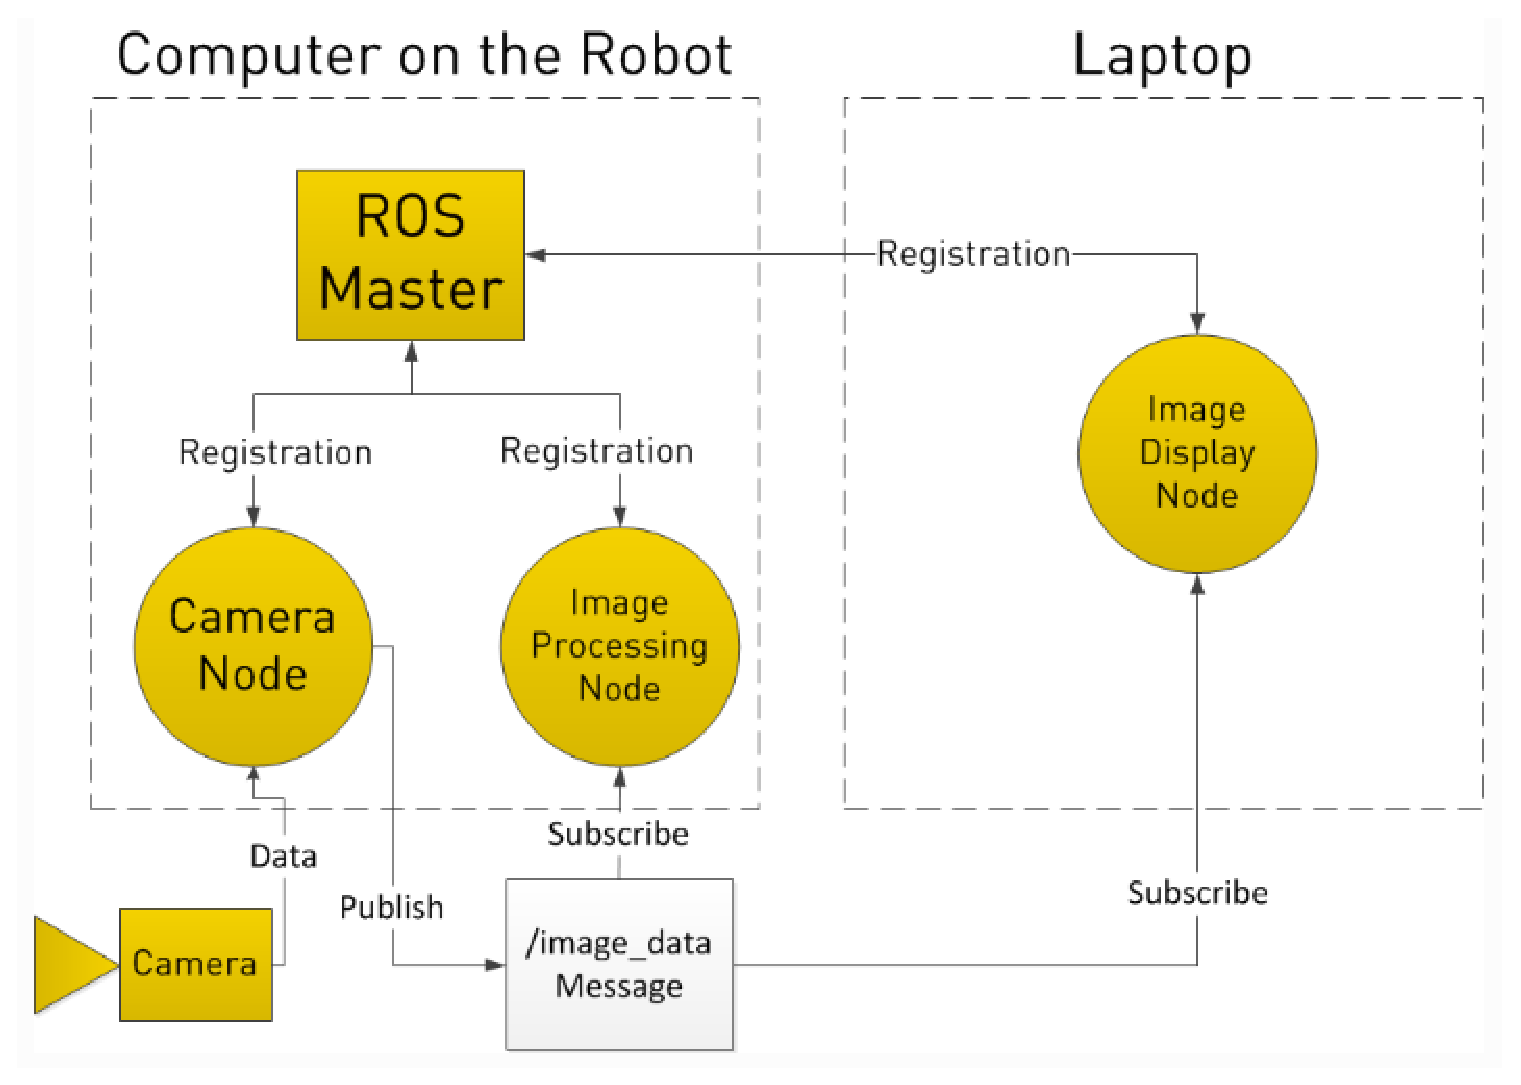
\includegraphics[width=0.8\textwidth]{images/cap3/RosDiagrama.eps}
    \captionof{figure}{Ejemplo de captura de imágenes}
    \label{fig:Ros-Diagram}
\end{minipage}

%+++++++++++++++++++++++++++++++++++++++++++++++++++++++++++++++++++++++++++++++
\subsection{Características}
% http://www.ros.org/core-components/

ROS proporciona un gran número de librerías para resolver los problemas comunes
en el desarrollo robótico con el objetivo de simplificar el la dura carga de
tiempo y trabajo que eso supone. Estas son algunas de las principales
características:

\begin{itemize}
  \item \textbf{Mensajes estándar:} existe una gran variedad de mensajes básicos
  ya definidos para la mayoría de tareas del robot como la pose, coordenadas de
  transformación, sensores, odometría, mapas, etc. 
  \item \textbf{Geometría del robot:} la librería 'tf' se encarga de detectar
  las diferentes partes de un robot frente al resto de ellas, siendo posible
  coordinar y transformar más de cien grados de libertad.
  \item \textbf{Lenguaje de descripción:} ROS permite describir las
  particularidades de un robot de una manera redactable. Para ello se usa URDF
  (Unified Robot Description Format), un lenguaje de descripción basado en XML
  que describe todas las características físicas del robot como el tamaño de las
  ruedas, la distancia entre los diferentes componentes e incluso la apariencia
  visual de cada elemento.
  \item \textbf{Diagnóstico:} se ha diseñado un sistema capaz de recoger toda la
  información del robot, para poder registrar, analizar y resolver cualquier
  problema presente en el estado del robot.
  \item \textbf{Navegación:} la mayoría de problemas en la navegación de un
  robot como la estimación de la pose, la localización en un mapa y la
  construcción del misma, son fácilmente resolubles mediante los paquetes que
  proporciona ROS sin necesidad de buscar soluciones propias o de terceros.
\end{itemize}

%+++++++++++++++++++++++++++++++++++++++++++++++++++++++++++++++++++++++++++++++
\subsection{Herramientas}
% http://www.ros.org/core-components/
Una de las características más importantes de ROS está en las herramientas de
desarrollo disponibles. Existe una gran variedad de software de todo tipo:
visualización, depuración, resumen del estado, etc. Gracias al mecanismo de
publicación/suscripción es muy sencillo observar y depurar lo que está
ocurriendo en todo momento.

Por otra parte, ROS puede ser utilizado sin necesidad de usar una interfaz
gráfica (GUI). Toda las características y funcionalidades de ROS pueden
realizarse a través de más de 45 comandos en consola: lanzar grupos de nodos,
examinar tópicos y servicios, grabar y reproducir bolsas de datos, etc. En
cualquier otro caso existe una importante variedad de herramientas con interfaz
gráfica que extienden la funcionalidad de estos comandos. A continuación se
pueden ver algunos de ellos.

% http://introlab.github.io/rtabmap/
%--------------------------------------
\paragraph{RTAB-Map ROS} \hspace{0pt}

Esta herramienta es una extensión del software original RTAB-Map. RTAB-Map
es un aprovechamiento de las técnicas de SLAM capaz de detectar los cierres de
bucles en la navegación de un robot a partir de la apariencia de las imágenes,
los cuales son registrados en un grafo que representa el mapa. Por otra parte,
permite la reconstrucción tridimensional del mapa, el cuál es representado como
una nube de puntos. 

ROS cuenta con RTABMapviz para visualizar de forma gráfica el resultado de la
detección de los cierres de bucle y la generación en vivo del mapa
tridimensional.

%--------------------------------------
\paragraph{RViz} \hspace{0pt}

RViz es una herramienta de propósito general que permite visualizar en un
espacio tridimensional mucho de los elementos de un robot como ruedas, brazos o
sensores láser. RViz también puede visualizar diferentes mensajes comunes de ROS
como barridos láser, nube de puntos, las imágenes de las cámaras o también con
la posibilidad de mostrar el mapa del entorno (previamente almacenado).

RViz también puede interactuar con la información de la biblioteca 'tf' para
mostrar toda la información del sistema de coordenadas de los sensores desde
diferentes perspectivas. Entre las ventajas, destaca que se trata de una
herramienta muy importante ya que permite visualizar que ocurre en el robot en
cada momento en busca de errores.

%--------------------------------------
\paragraph{RQt} \hspace{0pt}

RQt es un framework escrito en Qt como el nombre indica que permite desarrollar
aplicaciones personalizadas con interfaz gráfica para cualquier robot. RQt trae
consigo una gran variedad de plugins y/o utilidades para trabajar, de esta forma
cualquier usuario puede modificar según sus necesidades la apariencia y
distribución de estos. Aunque también es posible escribir nuevos plugins
ajustados a la medida de cualquier usuario.

Entre los principales plugins, destacan:

\begin{itemize}
  \item \textbf{rqt\_image\_view:} se trata de la adaptación del paquete de ROS
  'image\_view. Permite visualizar todas las imágenes disponibles en los
  diferentes tópicos activos, tanto imágenes normales, como imágenes en
  estéreo e imágenes de disparidad.
  \item \textbf{rqt\_bag:} permite grabar y gestionar bolsas de datos. Una bolsa
  en formato que permite almacenar todos tipo de datos previamente grabados como
  la lectura de sensores, las imágenes capturadas o el sistema de coordenadas
  utilizado. Son de gran utilidad para depurar y comparar con otras bolsas, ya
  que se pueden visualizar siempre que se deseen sin necesidad de utilizar el
  robot que se utilizó.
  \item \textbf{rqt\_graph:} muestra el estado actual del sistema en forma de
  grafo, como los nodos y las conexiones entre ellos, siendo de gran utilidad
  para la depuración de errores ya que son una forma rápida de ver que todo está
  el sistema está conectado correctamente.
  \item \textbf{rqt\_reconfigure:} adaptación del paquete 'dynamic\_reconfigure'
  que que permite modificar en tiempo real todos los parámetros de los nodos,
  para realizar modificaciones rápidas al vuelo. La configuración de los
  parámetros se puede exportar para utilizar en el futuro.
\end{itemize}

%+++++++++++++++++++++++++++++++++++++++++++++++++++++++++++++++++++++++++++++++




%%%%%%%%%%%%%%%%%%%%%%%%%%%%%%%%%%%%%%%%%%%%%%%%%%%%%%%%%%%%%%%%%%%%%%%%%%%%%%%

\chapter{Desarrollo}
\label{chapter:cuatro}

%%%%%%%%%%%%%%%%%%%%%%%%%%%%%%%%%%%%%%%%%%%%%%%%%%%%%%%%%%%%%%%%%%%%%%%%%%%%%%%
% Chapter 4 : Desarrollo
%%%%%%%%%%%%%%%%%%%%%%%%%%%%%%%%%%%%%%%%%%%%%%%%%%%%%%%%%%%%%%%%%%%%%%%%%%%%%%%


Los capítulos intermedios servirán para cubrir los siguientes aspectos:
antecedentes, problemática o estado del arte, objetivos, fases y desarrollo del proyecto.


%++++++++++++++++++++++++++++++++++++++++++++++++++++++++++++++++++++++++++++++

En el capítulo ~\ref{chapter:intro} se describió bla, bla, bla.....




%%%%%%%%%%%%%%%%%%%%%%%%%%%%%%%%%%%%%%%%%%%%%%%%%%%%%%%%%%%%%%%%%%%%%%%%%%%%%%%
\newpage{\pagestyle{empty}}
\thispagestyle{empty}

\chapter{Conclusiones y líneas futuras}
\label{chapter:Conclusiones}

%%%%%%%%%%%%%%%%%%%%%%%%%%%%%%%%%%%%%%%%%%%%%%%%%%%%%%%%%%%%%%%%%%%%%%%%%%%%%
% Chapter 5: Conclusiones y Trabajos Futuros 
%%%%%%%%%%%%%%%%%%%%%%%%%%%%%%%%%%%%%%%%%%%%%%%%%%%%%%%%%%%%%%%%%%%%%%%%%%%%%%%

%+++++++++++++++++++++++++++++++++++++++++++++++++++++++++++++++++++++++++++++++
\section{Conclusiones}
\label{5:sec:1}
%%%%%%%%%%%%%%%%%%%%%%%%%%%%%%%%%%%%%%%%%%%%%%%%%%%%%%%%%%%%%%%%%%%%%%%%%%%%%
% Chapter 5: Conclusiones y Líneas Futuras 
%%%%%%%%%%%%%%%%%%%%%%%%%%%%%%%%%%%%%%%%%%%%%%%%%%%%%%%%%%%%%%%%%%%%%%%%%%%%%%%

%+++++++++++++++++++++++++++++++++++++++++++++++++++++++++++++++++++++++++++++++
% \section{Conclusiones}
% \label{5:sec:1}

En este trabajo se ha visto que las cámaras estereoscópicas permiten obtener
unas imágenes del mundo que le rodea muy próximas a la realidad. Por sí sola, la
odometría visual de este tipo de cámaras funciona muy bien en la mayoría de
situaciones, tanto en espacios cerrados como en lugares más abiertos, siendo un
claro competidor del sistema actual de la silla Perenquén, el uso de una cámara
RGB-D. Por otro lado, es importante mencionar que la integración de sensores
mecánicos y sensores láser permite corregir algunos de los problemas que son
propensos a ocurrir cuando las ocasiones lumínicas no son las idóneas.

Es necesario recordar, que es muy difícil recoger con exactitud la información
de la naturaleza, el entorno que nos rodea está vivo, sin embargo, la visión
estereoscópica sirve de pilar, junto con otros sensores para obtener la mayor
aproximación posible del mundo.

%+++++++++++++++++++++++++++++++++++++++++++++++++++++++++++++++++++++++++++++++


%+++++++++++++++++++++++++++++++++++++++++++++++++++++++++++++++++++++++++++++++
\section{Líneas futuras}
\label{5:sec:2}
%%%%%%%%%%%%%%%%%%%%%%%%%%%%%%%%%%%%%%%%%%%%%%%%%%%%%%%%%%%%%%%%%%%%%%%%%%%%%
% Chapter 5: Conclusiones y Líneas Futuras
%%%%%%%%%%%%%%%%%%%%%%%%%%%%%%%%%%%%%%%%%%%%%%%%%%%%%%%%%%%%%%%%%%%%%%%%%%%%%%%

%+++++++++++++++++++++++++++++++++++++++++++++++++++++++++++++++++++++++++++++++
% \section{Líneas futuras}
% \label{5:sec:2}

Más allá de la reconstrucción del mapa en 3D y la localización en el mismo, el
siguiente punto más atractivo es la detección y posterior esquiva de los
obstáculos en el camino del robot. Con este objetivo cumplido, el robot podría
navegar de forma autónoma.

Por otro lado, en función de los buenos resultados con la visión estéreo, se
debería analizar que otros sistemas alternativos a PlayStation Camera existen.

%+++++++++++++++++++++++++++++++++++++++++++++++++++++++++++++++++++++++++++++++


%+++++++++++++++++++++++++++++++++++++++++++++++++++++++++++++++++++++++++++++++


%%%%%%%%%%%%%%%%%%%%%%%%%%%%%%%%%%%%%%%%%%%%%%%%%%%%%%%%%%%%%%%%%%%%%%%%%%%%%%%
\newpage{\pagestyle{empty}}
\thispagestyle{empty}

\chapter{Summary and Conclusions }
\label{chapter:ingles}

%%%%%%%%%%%%%%%%%%%%%%%%%%%%%%%%%%%%%%%%%%%%%%%%%%%%%%%%%%%%%%%%%%%%%%%%%%%%%
% Chapter 6: Summary and Conlusions
%%%%%%%%%%%%%%%%%%%%%%%%%%%%%%%%%%%%%%%%%%%%%%%%%%%%%%%%%%%%%%%%%%%%%%%%%%%%%%%

%++++++++++++++++++++++++++++++++++++++++++++++++++++++++++++++++++++++++++++++

This chapter is compulsory.
The memory should include an extended summary and conclusions in english. 

%---------------------------------------------------------------------------------
\section{First Section}
\label{6:sec:1}



%%%%%%%%%%%%%%%%%%%%%%%%%%%%%%%%%%%%%%%%%%%%%%%%%%%%%%%%%%%%%%%%%%%%%%%%%%%%%%%
\newpage{\pagestyle{empty}}
\thispagestyle{empty}

\chapter{Presupuesto}
\label{chapter:Presupuesto}

%%%%%%%%%%%%%%%%%%%%%%%%%%%%%%%%%%%%%%%%%%%%%%%%%%%%%%%%%%%%%%%%%%%%%%%%%%%%%
% Chapter 7: Presupuesto
%%%%%%%%%%%%%%%%%%%%%%%%%%%%%%%%%%%%%%%%%%%%%%%%%%%%%%%%%%%%%%%%%%%%%%%%%%%%%%%

%++++++++++++++++++++++++++++++++++++++++++++++++++++++++++++++++++++++++++++++

Este capítulo es obligatorio.
Toda memoria de Trabajo de Fin de Grado debe incluir un presupuesto.

%---------------------------------------------------------------------------------
\section{Sección Uno}
\label{7:sec:1}


%--------------------------------------------------------------------------
\begin{table}[!ht]
\begin{center}
\begin{tabular}{|p{25mm}|p{80mm}|} \hline 
\textbf{Tipos } & \textbf{Descripcion} \\ \hline
AAAA &
BBBB
\\
\hline

CCCC &
DDDD
\\
\hline

EEEE &
FFFF
\\
\hline

GGGG &
HHHH
\\
\hline

\end{tabular}
\end{center}
\caption{Tabla resumen de los Tipos}
\label{table:resOthers}
\end{table}






%%%%%%%%%%%%%%%%%%%%%%%%%%%%%%%%%%%%%%%%%%%%%%%%%%%%%%%%%%%%%%%%%%%%%%%%%%%%%%%

%%%%%%%%%%%%%%%%%%%%%%%%%%%%%%%%%%%%%%%%%%%%%%%%%%%%%%%%%%%%%%%%%%%%%%%%%%%%%%%
\newpage{\pagestyle{empty}}
\thispagestyle{empty}
\begin{appendix}

\chapter{Título del Apéndice 1}
\label{appendix:1}
\section{Algoritmo XXX}
\label{Apendice1:XXX}

\begin{center}
\begin{footnotesize}
\begin{verbatim}

***********************************************************************************
*
* Fichero .h
*
***********************************************************************************
*
* AUTORES
*   
*
* FECHA
*   
*
* DESCRIPCION
*   
*
************************************************************************************/

\end{verbatim}
\end{footnotesize}
\end{center}

\section{Algoritmo YYY}
\label{Apendice1:YYY}

\begin{center}
\begin{footnotesize}
\begin{verbatim}


/***********************************************************************************
 *
 * Fichero .h
 *
 ***********************************************************************************
 *
 * AUTORES
 *
 * FECHA
 *
 * DESCRIPCION
 *
 *
 ************************************************************************************/

\end{verbatim}
\end{footnotesize}
\end{center}


\chapter{Título del Apéndice 2}
\label{appendix:2}
\section{Otro apéndice: Sección 1}
\label{Apendice2:label}

\begin{center}
\begin{footnotesize}

\begin{verbatim}
Texto
\end{verbatim}

\end{footnotesize}
\end{center}

\section{Otro apéndice: Sección 2}
\label{Apendice2:label2}

\begin{center}
\begin{footnotesize}

\begin{verbatim}
Texto
\end{verbatim}


\end{footnotesize}
\end{center}


\end{appendix}

%%%%%%%%%%%%%%%%%%%%%%%%%%%%%%%%%%%%%%%%%%%%%%%%%%%%%%%%%%%%%%%%%%%%%%%%%%%%%%%
\addcontentsline{toc}{chapter}{Bibliografía}
\bibliographystyle{plain}

\bibliography{memtfg}
\nocite{*}

%%%%%%%%%%%%%%%%%%%%%%%%%%%%%%%%%%%%%%%%%%%%%%%%%%%%%%%%%%%%%%%%%%%%%%%%%%%%%%%

\end{document}
